\documentclass[Lau, noexaminfo, oneside]{sapthesis} %to print the book, twoside
\usepackage[utf8]{inputenc}
\usepackage[italian]{babel}
\usepackage{amssymb}
\usepackage{float}
\usepackage{hyperref}
\usepackage{cite}
\usepackage{enumitem}
\usepackage{microtype}

\title{Simulazione del modello di Ising mediante una Rete Generativa Avversaria}
\author{Ruben Gargiulo}
\date{}
\IDnumber{1824800}
\course{Fisica}
\courseorganizer{Facoltà di Scienze Matematiche, Fisiche e Naturali}
\submitdate{2019/2020}
\copyyear{2020}
\advisor{Prof. S.Giagu}
\authoremail{gargiulo.1824800@studenti.uniroma1.it}
\begin{document}

\frontmatter
\maketitle

\begin{abstract}
Negli ultimi anni le reti neurali convoluzionali si sono affermate come uno dei metodi più efficaci per rappresentare ed analizzare dati complessi, soprattutto se strutturati come immagini. Al contempo le GAN (reti generative avversarie) hanno ampliato il potere delle reti neurali permettendo di generare nuovi campioni dei dataset di partenza.
I modelli generativi formati da reti avversarie convoluzionali, detti DCGAN, uniscono questi due aspetti dando accesso a simulazioni fisiche sempre più realistiche. Uno dei punti vincenti di quest'approccio è che, una volta allenate le reti, la simulazione avviene in un tempo irrisorio rispetto a quello richiesto dai metodi tradizionali. In questa dissertazione discuterò dell'uso di una DCGAN per generare campioni 28x28 del modello di Ising, dato un certo range di temperatura.
\end{abstract}
\tableofcontents
\mainmatter
\chapter{Introduzione}
In fisica c'è una continua necessità di effettuare simulazioni numeriche. Esse possono porsi come veri e propri esperimenti virtuali, facilitando la comprensione dei fenomeni in studio, estendendo i limiti dei metodi sperimentali e consentendo di confutare alcune teorie o di formularne altre. \\
Molto spesso le simulazioni permettono di studiare fenomeni che non hanno una soluzione analitica, come nel caso della prima simulazione fisica di grande dimensione, effettuata nell'ambito del progetto Manhattan.
Per modellizzare il processo della detonazione nucleare, infatti, Fermi e i suoi collaboratori ne simularono il comportamento su grossi calcolatori analogici. In questa circostanza fu sviluppato da N. C. Metropolis l'algoritmo Monte Carlo, il metodo principe della simulazione fisica. A Metropolis dobbiamo anche l'invenzione dell'algoritmo più diffuso appartenente a questa classe, che porta infatti il suo nome.\\
Uno dei fenomeni più interessanti che normalmente si simula attraverso tale procedura è il ferromagnetismo. Esso è stato modellizzato per la prima volta, attraverso una catena di spin interagenti, da Ernst Ising, che non riscontrò transizioni di fase. In due e in tre dimensioni, al contrario, si osserva una transizione che corrisponde al passaggio dal ferromagnetismo al paramagnetismo dopo il superamento della temperatura di Curie: questo comportamento può essere osservato sperimentalmente anche con materiali di uso comune, come nel celebre Pendolo di Curie. \\
Il modello di Ising, inoltre, ha avuto un'importanza storica nell'affermazione della meccanica statistica moderna.
Già nel IV secolo a.C. Democrito notò che l'atomismo poteva spiegare i comportamenti discontinui della natura, ossia le transizioni di fase. Egli pensava che piccoli cambiamenti nel comportamento della materia su scala atomica potessero provocare modifiche osservabili nello stato macroscopico. 
Al contrario molti altri filosofi, la cui tesi si impose rimanendo dominante fino almeno al XIX secolo, erano convinti della natura continua della realtà (si ricordi il "Natura non facit saltus" di Leibniz). \\
Quando nell'Ottocento le leggi chimiche dimostrarono chiaramente l'esistenza degli atomi, J.Maxwell e L. Boltzmann applicarono le leggi meccaniche alla dinamica degli atomi e scoprirono che derivandone il comportamento collettivo si ottenevano le leggi dei gas, fondando così la meccanica statistica. Non tutti gli studiosi condividevano a pieno quest'approccio: negli anni '30 alcuni critici
(tra cui H. A. Kramers), basandosi sull'analiticità della funzione di partizione di un sistema finito, ritenevano fosse impossibile giustificare le transizioni di fase con la meccanica statistica. \cite{Kadanoff2009} \\
Lo studio del modello di Ising, al contrario, mostrò che la convergenza al limite termodinamico è così veloce che anche per reticoli piccoli si osservano transizioni di fase molto ripide.\\
Il modello di Ising in 2D ha una soluzione analitica proposta da Onsager (1948) e dimostrata da Yang (1952). Nonostante ciò, uno dei modi più affermati per visualizzare il modello e studiarne le proprietà è la simulazione numerica attraverso il metodo di Metropolis; esso però richiede molte iterazioni, per ciascuna configurazione generata, per giungere all'equilibrio. \\
Un metodo per velocizzare di molto la generazione di configurazioni del modello di Ising è quello di allenare una rete neurale a estrarre campioni da una distribuzione di probabilità che sia molto simile a quella voluta. Il sampling tramite la rete neurale già allenata, a differenza dell'algoritmo di Metropolis, non richiede nessuna iterazione. Esso infatti avviene generando dei numeri random e passandoli come argomento ad una funzione deterministica. Come tale, esso richiede una quantità sensibilmente minore di tempo e risorse di calcolo. Questa maggiore efficienza è dovuta al fatto che, con l'algoritmo di Metropolis, si ricostruisce ogni volta da capo la distribuzione voluta; al contrario, la rete apprende la distribuzione \textit{una tantum}. \\
Per verificare le potenzialità di quest'approccio, ho sviluppato una Deep Convolutional Generative Adversarial Network. Essa è formata da due reti neurali convoluzionali contrapposte: una (denominata discriminatrice) si allena a distinguere le configurazioni appartenenti al dataset da quelle generate dall'avversaria, l'altra (detta generatrice) si allena ad ingannare la rete discriminatrice. Effettuando il training delle due reti, ho costruito una DCGAN che, data una classe (tra 10 di temperatura) genera configurazioni credibili del modello di Ising. Inoltre i campioni fake estratti non presentano alcuni difetti presenti nel dataset di partenza, generato con l'algoritmo di Metropolis, dovuti al basso numero di iterazioni.
\chapter{Modello di Ising}
Il modello di Ising consiste, a livello geometrico, in un insieme di punti su un reticolo D-dimensionale. Per ogni punto $k$ c'è una variabile discreta $\sigma_k$ con valori $\lbrace-1, 1\rbrace$. Per ciascuna coppia di punti $i$ e $j$ c'è un termine di interazione $J_{ij}$. Inoltre al reticolo viene applicato un campo magnetico esterno $h_{k}$. L'energia di una data configurazione ha la forma:
\begin{equation}
H = - \sum_{i,j \text{ vicini}} J_{ij} \sigma_i \sigma_j - \sum_i h_i \sigma_i \,.
\label{isingcompleto}
\end{equation}
La prima somma si estende solo sulle coppie di punti contigui, ossia che differiscono di un vettore con modulo pari al passo reticolare. Spesso, come nel nostro caso, il modello di Ising si analizza nell'ipotesi che non ci sia campo esterno e che l'interazione $J$ non vari con la posizione:
\begin{equation}
H = -J \sum_{i,j \text{ vicini}}  \sigma_i \sigma_j \,.
\end{equation}
Il modello è stato introdotto per analizzare il comportamento ferromagnetico della materia, con $\sigma_{i}$ che rappresenta la proiezione dello spin su un asse. Nella forma semplificata, il ground state consiste in una configurazione con $\sigma$ tutti uguali. In due dimensioni, a causa delle fluttuazioni termiche, le configurazioni osservate presentano comportamenti diversi al variare della temperatura. Il modello è stato infatti storicamente il primo ad esibire una transizione di fase continua da situazioni ordinate a disordinate in corrispondenza di una precisa temperatura.
Si distinguono infatti, a livello qualitativo:
\begin{itemize}
\item configurazioni ordinate, in cui gli spin sono quasi tutti uguali, a bassa temperatura;
\item configurazioni critiche, in cui gli spin tendono ad organizzarsi in cluster, a temperature vicine a quella critica;
\item configurazioni disordinate, in cui gli spin sono organizzati in modo random, similmente all'effetto neve, ad alta temperatura.
\end{itemize}
Il parametro d'ordine che consente facilmente di analizzare la transizione è la cosiddetta magnetizzazione spontanea. Essa rappresenta la media di tutti i valori degli spin e si calcola a partire dalla temperatura con la formula esatta di Onsager \cite{onsager}:
\begin{equation}
|M|(\beta) = (1-\sinh(2\beta J)^{-4})^{1/8} \,.
\label{eqonsager}
\end{equation}
\begin{figure}[H]
\fbox{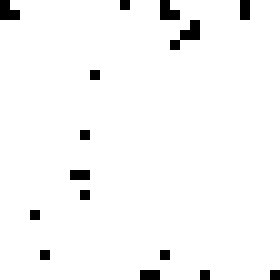
\includegraphics[scale=0.35]{ord.png}}
\hspace{10pt}
\fbox{
\includegraphics[scale=0.35]{crit.png}}
\hspace{10pt}
\fbox{
\includegraphics[scale=0.35]{disord.png}}
\centering
\caption{Configurazioni, rispettivamente, ordinate, critiche e disordinate del modello semplificato.}
\end{figure}
\section{Approssimazione di campo medio}
La dimostrazione della formula di Onsager si ricava tramite un procedimento lungo e laborioso; pertanto, per cogliere gli aspetti salienti del comportamento dell'hamiltoniana, è preferibile utilizzare un'approssimazione di campo medio\cite{meanfield}. Sia $m$ la media degli spin su tutto il reticolo (che supponiamo bidimensionale e quadrato) e $\delta\sigma_k = \sigma_k - m$. Si ha dunque:
\begin{equation}
H = -\sum_{i,j \text{ vicini}}  (m + \delta\sigma_i)(m + \delta\sigma_j) - \sum_i h_i \sigma_i \,,
\end{equation}
avendo posto (come sarà anche nella trattazione della GAN) $J=1$.
Trascurando i termini quadratici in $\delta\sigma_{i,j}$ si ricava:
\begin{equation}
H = - \sum_{i,j \text{ vicini}}  [m^2 + m (\delta\sigma_i + \delta\sigma_j)] - \sum_i h_i \sigma_i \,.
\end{equation}
Indicando con $nn(k)$ i 4 siti primi vicini del sito k-esimo si può scrivere:
\begin{equation}
\sum_{i,j \text{ vicini}} = \frac{1}{2} \sum_i \sum_{j\in nn(i)} = \frac{1}{2} \sum_j \sum_{i\in nn(j)} \,.
\end{equation}
Riscrivendo l'hamiltoniana in questa notazione:
\begin{equation}
H = \frac{1}{2} \sum_i \sum_{j\in nn(i)} m^2 - \frac{1}{2}m \sum_i \sum_{j\in nn(i)} \sigma_i - \frac{1}{2}m \sum_j \sum_{i\in nn(j)} \sigma_j - \sum_i h_i \sigma_i \,.
\end{equation}
Invertendo $i$ e $j$ nel penultimo addendo e sommando si ottiene:
\begin{equation}
H = 2 N m^2 - (4 m+h) \sum_i \sigma_i \,.
\end{equation}
Si vede inoltre, confrontando con l'eq. \eqref{isingcompleto} che la quantità $h_{eff} = h+4m$ ha il ruolo di un campo magnetico.
Essendo stata eliminata l'interazione spin-spin, si può scrivere l'hamiltoniana di singola particella:
\begin{equation}
H_i =  2  m^2 - h_{eff} \sigma_i \,.
\label{hamiltonianasingola}
\end{equation}
La funzione di partizione del sistema vale quindi (avendo posto $k_{B} = 1$):
\begin{equation}
Z = \frac{1}{N!} \left [ \sum_{\sigma \in \lbrace{1,\,-1}\rbrace} \exp \lbrace -2 \beta m^2 +  \beta h_{eff} \sigma \rbrace \right ] ^N \,,
\end{equation}
ossia:
\begin{equation}
Z = \frac{2^N}{N!} \exp \lbrace - 2 \beta  N m^2 \rbrace \cosh^N(\beta h_{eff}) \,.
\end{equation}
Calcoliamo ora $m$ a partire da $Z$:
\begin{equation}
m = \frac{1}{N} \sum_i \langle \sigma_i \rangle \,.
\end{equation}
Lo spin medio su ogni sito si trova mediando su tutte le configurazioni $S$:
\begin{equation}
\sum_i \langle \sigma_i \rangle = \frac{1}{Z} \sum_{S} \sum_i \sigma_i  \exp\lbrace-\beta H(S)\rbrace \,.
\end{equation}
Dalla \eqref{hamiltonianasingola} notiamo che:
\begin{equation}
\frac{\partial H}{\partial h_{eff}} = - \sum_i \sigma_i \,,
\end{equation}
da cui:
\begin{equation}
m = - \frac{1}{NZ} \sum_{S} \frac{\partial H(S)}{\partial h_{eff}} \exp\lbrace-\beta H(S)\rbrace = \frac{1}{\beta NZ} \frac{\partial}{\partial h_{eff}} \sum_{S} \exp\lbrace-\beta H(S)\rbrace \,.
\end{equation}
Si ottiene infine un'equazione di autoconsistenza:
\begin{equation}
m = \frac{1}{\beta N} \frac{\partial \ln(Z)}{\partial h_{eff}} = \tanh(\beta h_{eff})= \tanh(h+4\beta m) \,.
\end{equation}
L'equazione ottenuta è di tipo trascendente, ma può essere risolta graficamente.
Poiché vogliamo studiare la magnetizzazione spontanea, poniamo $h=0$; in tal caso per $4\beta<1$ l'unica soluzione è $m=0$, di conseguenza non c'è ferromagnetismo. Invece per $4\beta>1$ vi sono anche due soluzioni opposte diverse da 0, dunque si osserva una magnetizzazione spontanea.
Il comportamento ottenuto è quindi qualitativamente corretto, dal punto di vista magnetico: lo svantaggio dell'approssimazione risiede nell'errata temperatura critica predetta, se confrontata con quella all'eq. \eqref{eqonsager}.
\section{Simulazione attraverso l'algoritmo di Metropolis}
La probabilità di ciascuna configurazione di $N$ spin $\sigma = [\sigma_1, \sigma_2, ..., \sigma_N]$ è data dalla distribuzione di Boltzmann:
\begin{equation}
P_{\beta }(\sigma)={\frac {e^{-\beta H(\sigma )}}{\sum\limits_{\sigma} e^{-\beta H(\sigma )}}} \,.
\end{equation}
Dunque il rapporto tra le probabilità di due configurazioni $\sigma_1$, $\sigma_2$ è:
\begin{equation}
\frac{P_{\beta }(\sigma_1)}{P_{\beta }(\sigma_2)} = e^{-\beta [H(\sigma_1) - H(\sigma_2)]} \,.
\end{equation}
La simulazione tradizionale del modello di Ising avviene attraverso l'algoritmo di Metropolis su un reticolo bidimensionale $L \times L$.
Esso consiste in una serie di modifiche progressive della configurazione, da quella iniziale a quella finale. \\Per ogni iterazione, partendo da una configurazione $A$ si determina casualmente un sito $k$ sul reticolo e si inverte $\sigma_k$, ottenendo una configurazione $B$. Se l'energia dopo l'inversione diminuisce si accetta la nuova configurazione $B$, altrimenti la si accetta con probabilità $e^{\beta (H_A - H_B)}$. Nel calcolo dell'energia, per evitare effetti di bordo, si usano condizioni al contorno periodiche. Dopo un certo numero di iterazioni si ottiene infine una configurazione di equilibrio. \cite{metropolis-hastings}
\section{Approfondimento: applicazioni computazionali}
Il modello di Ising, nella sua forma completa
\begin{equation}
H = - \sum_{i,j \text{ vicini}} J_{ij} \sigma_i \sigma_j - \sum_i h_i \sigma_i
\end{equation}
è uno dei modelli fisici più usati al di fuori del suo ambito. Si stima che nel periodo tra il 1969 al 1997 siano stati pubblicati più di 12,000 articoli nei quali lo si usava per descrivere fenomeni in diversi campi, dall'intelligenza artificale alla zoologia. \cite{dwave}
Un'interessante applicazione riguarda il calcolo booleano parallelo. Infatti a bassissima temperatura, assegnata una matrice $J$ e un vettore $h$, le configurazioni che si osservano in natura sono quelle che corrispondono al minimo globale dell'energia. La natura quindi provvede autonomamente all'ottimizzazione dei valori $\sigma$ per minimizzare $H$, che è un problema computazionalmente NP-completo, ossia molto dispendioso da calcolare. A questo punto si può introdurre un'analogia tra il calcolo di espressioni booleane e la minimizzazione di $H$. Trattando $\sigma=-1, 1$ come un valore booleano falso o vero, le tavole della verità per gli operatori logici possono essere codificate attraverso modelli di Ising, variando $J$ e $h$.\\ Introducendo il concetto di soddisfacibilità booleana (SAT), che consiste nel determinare, data una espressione booleana, se esiste un qualche assegnamento di valori 1 e 0 tali da rendere l'intera espressione vera, un problema SAT si può rappresentare con un modello di Ising cosicchè un espressione è soddisfacibile solo se lo stato fondamentale del reticolo associato ha energia 0. Dunque un problema SAT può essere risolto fisicamente codificandolo attraverso un reticolo di spin a bassa temperatura ed osservando lo stato fondamentale. In questo modo si risolve il problema attraverso un calcolo estremamente parallelo (quantum annealing).\cite{quantumannealing}
\begin{table}[H]
\begin{tabular}{l|l}
Logic function & Ising function\\
\hline
$z = 0$        & 2$\sigma_z$                                                                                   \\
$z = x \wedge y$    & $-\sigma_x - \sigma_y + 2\sigma_z - 2\sigma_x\sigma_z - 2\sigma_y\sigma_z + \sigma_x\sigma_y$ \\
$z = x \wedge \lnot y$   & $-\sigma_x + \sigma_y + 2\sigma_z - 2\sigma_x\sigma_z + 2\sigma_y\sigma_z - \sigma_x\sigma_y$ \\
$z = x$        & $-2\sigma_x\sigma_z$                                                                          \\
$z = \lnot x \wedge y$   & $+\sigma_x - \sigma_y + 2\sigma_z + 2\sigma_x\sigma_z - 2\sigma_y\sigma_z - \sigma_x\sigma_y$ \\

$z = x \vee y $   & $\sigma_x + \sigma_y - 2\sigma_z - 2\sigma_x\sigma_z - 2\sigma_y\sigma_z + \sigma_x\sigma_y$  \\

\end{tabular}
\centering
\caption{Esempi di associazione tra equivalenze logiche (verificate nello stato fondamentale) ed energia dei reticoli \cite{quantumannealing}}
\end{table}
\chapter{Deep Learning}
\section{Introduzione alle Reti Neurali}
Una rete neurale artificiale consiste in un insieme di unità di calcolo elementari dette neuroni, collegate da canali di trasmissione dell'informazione detti sinapsi.
Il tipo di neurone più utilizzato è detto percettrone; esso è collegato da sinapsi a molteplici neuroni di input e ad un solo neurone di output. Rappresentando i valori in input come un vettore $x_{in}$ ed il valore in output come uno scalare $x_{out}$, l'uscita del percettrone corrisponde a:
\begin{equation}
x_{out} = \chi (w \cdot x_{in} + b) \,,
\end{equation}
dove $w$ (detto vettore dei pesi sinaptici) e $b$ (detto vettore dei bias) hanno la stessa dimensione di $x_{in}$ e $\chi$ è una funzione reale di variabile reale (detta funzione di attivazione).
\begin{figure}[H]
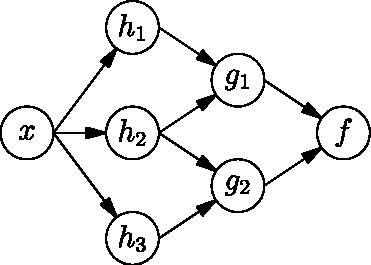
\includegraphics[width=0.3\textwidth]{grafo.pdf}
\centering
\caption{Schematizzazione tramite un grafo di una rete neurale composta da percettroni.}
\end{figure}
Le reti neurali più utilizzate, dette feedforward, sono organizzate in più strati (detti layer) di neuroni, che non presentano connessioni tra neuroni dello stesso strato e tra neuroni di strati non contingui.
La ragione del successo delle reti di questo tipo risiede nel teorema di approssimazione universale. Esso afferma che una rete feedforward completamente connessa, con larghezza o profondità arbitraria e funzione di attivazione non lineare, può approssimare qualsiasi funzione continua. L'apprendimento automatico svolto utilizzando tali reti, per la loro proprietà di "profondità" e per il fatto che sono capaci di rappresentare informazioni tramite gerarchie di concetti, è detto comunemente Deep Learning, o Deep Representation Learning.
\begin{figure}[H]
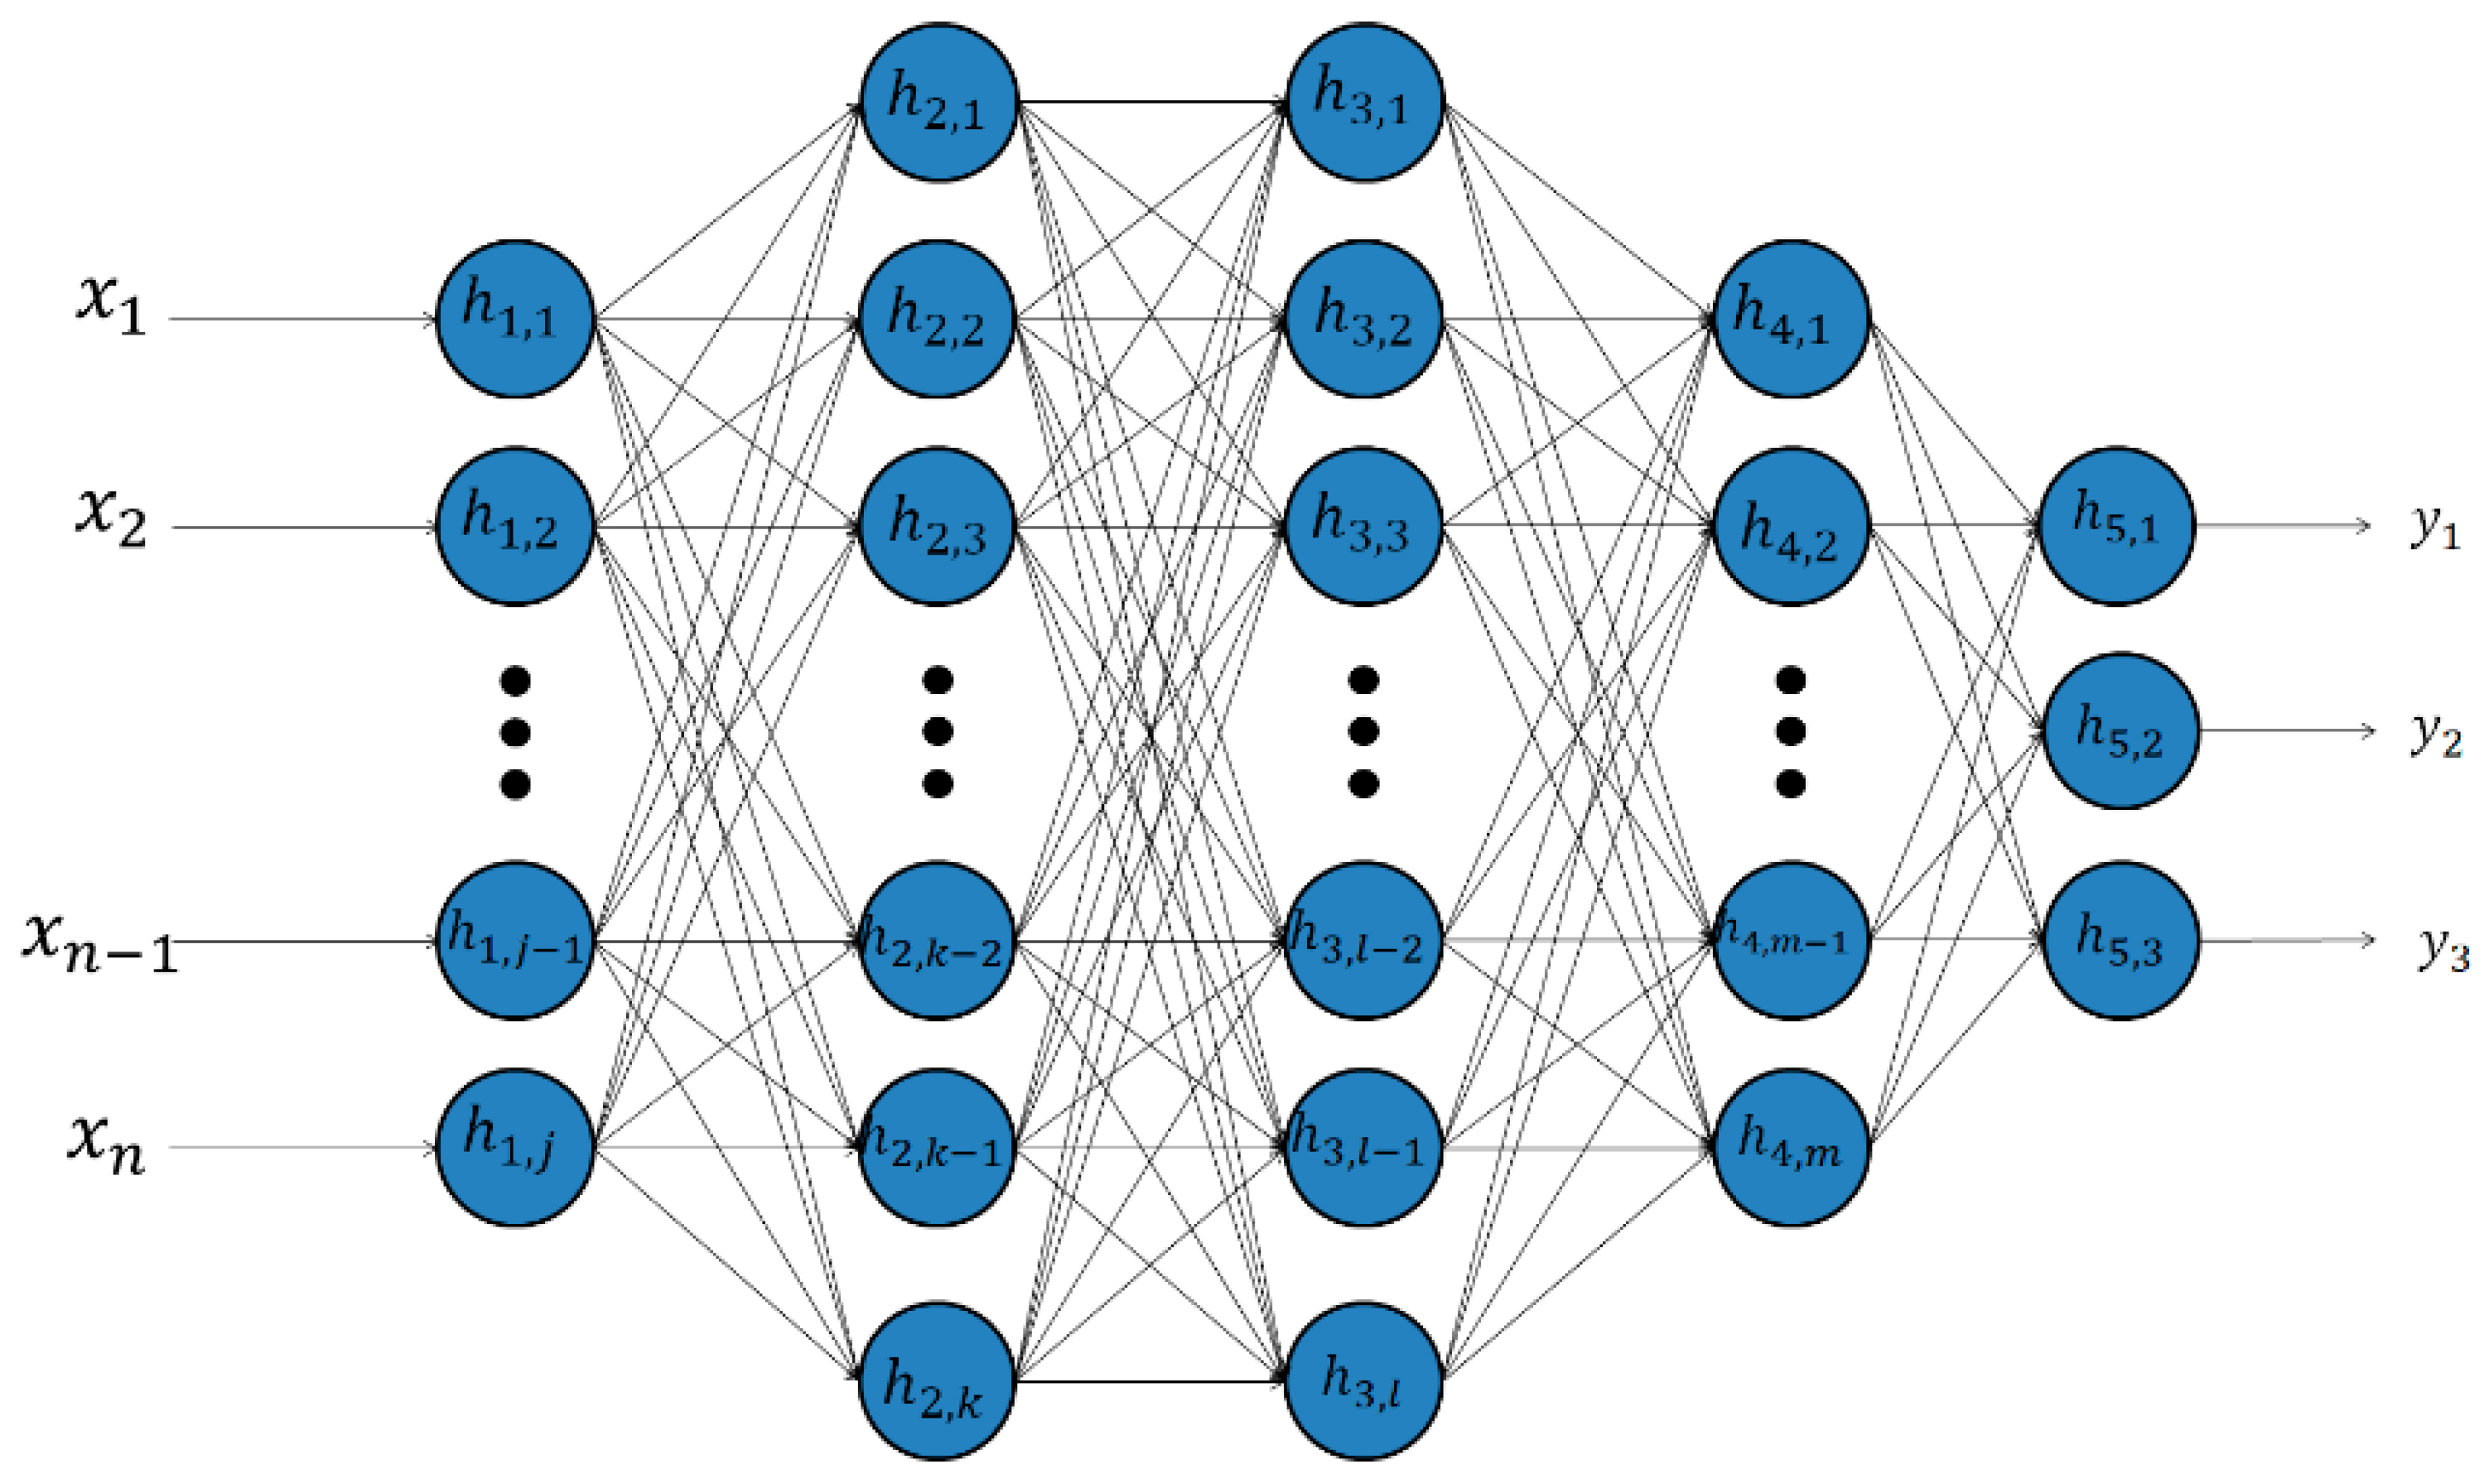
\includegraphics[width=0.7\textwidth]{information-10-00122-g002.png}
\centering
\caption{Schematizzazione tramite un grafo di una rete feedforward.}
\end{figure}
Il metodo standard per l'addestramento di queste reti consiste nel trovare, tramite discesa lungo il gradiente, i pesi e i bias che minimizzano una loss function, rappresentante la discrepanza tra gli output effettivi e quelli previsti.
\section{Formalismo matematico}
Denotiamo con $W_{jk}^l$ il peso sinaptico dal k-esimo neurone dello strato $l-1$ al j-esimo neurone dello strato $l$ e con $b^l_j$ il bias per il j-esimo neurone nello strato l-esimo, che ha come funzione di attivazione $f^l$.\\
L'output (detto anche attivazione) del neurone j-esimo dello strato l-esimo vale dunque:
\begin{equation}
a_j^l = f^l(\sum_k W_{jk}^l a_k^{l-1} + b_j^l) \,.
\label{attivazioni}
\end{equation}
Definiamo ora, a partire da $W_{jk}^l$ e $b^l_j$ una matrice $W^l$ (detta matrice dei pesi per lo strato l-esimo) ed un vettore $b^l$ (detto vettore dei bias per lo strato l-esimo).
Inoltre, a partire dalla funzione di attivazione $f^l$ dei neuroni dello strato l-esimo, definiamo due campi vettoriali $F^l$ ed $(F^l)'$ tali che:
\begin{align}
F^l_j(v) = f^l(v_j) \,,\\
(F^l)'_j(v) = (f^l)'(v_j) \,.
\end{align}
Dunque le attivazioni dei neuroni dello strato l-esimo, scritte in forma vettoriale, valgono:
\begin{equation}
a^l = F^l(W^l a^{l-1} + b^l) \,.
\end{equation}
L'output $y$ di una rete neurale di tipo feedforward $x$ si può quindi scrivere (nel caso privo di bias) come:
\begin{equation}
y = F^L (W^L F^{L-1}(W^{L-1} ... F^1 ( W^1 x ) ... )) \,.
\end{equation}
\section{Discesa lungo il gradiente}
L'algoritmo comunemente utilizzato per modificare pesi e bias minimizzando la funzione di costo è la cosiddetta discesa lungo il gradiente. Essa è una procedura di ottimizzazione, pubblicata per la prima volta da Cauchy nel 1847, che consente di minimizzare funzioni differenziabili reali. \\
La discesa consiste in un percorso a passi discreti sviluppato partendo da una posizione iniziale $\mathbf{w}_0$ nello spazio dei parametri e muovendosi ad ogni step con uno spostamento dato dal prodotto tra un parametro $\eta$ (detto learning rate) e l'opposto del gradiente della funzione di costo $C(\mathbf{w}, x)$ nel punto in cui ci si trova.\\
La procedura può essere schematizzata dal seguente pseudocodice (nel caso privo di bias):
\begin{align*}
& \text{initialize weigths } \mathbf{w}\\
& \textbf{for } k = 1,..., k_{max} \\
&\qquad \text{evaluate descent direction as average on dataset }\mathbf{x}\text{: } \\
& \qquad  \qquad \mathbf {p} _{k}:=- \langle \nabla C(\mathbf {w} _{k}, x) \rangle_{x \in \mathbf{x}}\\
&\qquad \mathbf {w} _{k+1}=\mathbf {w} _{k}+ \eta \, \mathbf {p} _{k}\\
&\textbf{end for}
\end{align*}
Durante l'addestramento di reti neurali si preferisce utilizzare una versione modificata dell'algoritmo, detta Stocastic Gradient Descent, nella quale si divide il dataset in più sottocampioni (detti mini-batch) che vengono utilizzati per il calcolo del gradiente medio. Ad ogni passo (detto epoca) si aggiornano i pesi ed i bias utilizzando in sequenza i gradienti medi ottenuti dai minibatch, come nel seguente pseudocodice (nel caso privo di bias):
\begin{align*}
& \text{initialize weigths } \mathbf{w}\\
& \text{split dataset into n mini-batches: }(\mathbf{x_1}, ..., \mathbf{x_n})\\
& \textbf{for } k = 1,..., k_{max} \\
& \qquad \textbf{for } i = 1,..., n \\
&\qquad \qquad {\text{evaluate descent direction as average on i-th mini-batch:}}\\
& \qquad \qquad \qquad \mathbf {p}:=- \langle \nabla C(\mathbf {w}, x)\rangle_{x \in \mathbf{x_i}} \\
&\qquad \qquad \mathbf {w}=\mathbf {w} + \eta \, \mathbf {p}\\
&\qquad \textbf{end for} \\
&\textbf{end for}
\end{align*} 
Tale metodo possiede maggiore stocasticità rispetto all'algoritmo naive e consente di ridurre la probabilità di intrappolamento all'interno di regioni di minimo locale durante la discesa.\\
Nell'utilizzo reale, tuttavia, si adottano metodi più sofisticati, che utilizzano anche i gradienti ai passi precedenti e variano il learning rate in modo da velocizzare il training (es. Adam, RMSProp ed altri).
\section{Backpropagation} 
La discesa lungo il gradiente non sarebbe praticabile a livello computazionale senza l'adozione della cosiddetta backpropagation. Essa consiste in una procedura per il calcolo dei gradienti della loss function rispetto ai pesi ed ai bias che riduce la complessità computazionale rispetto ad un approccio naive e consente di vettorizzare il codice relativo all'addestramento delle reti.\\
Per schematizzare tale metodo definiamo delle quantità ausiliarie, che rappresentano, rispettivamente, l'input allo strato l-esimo ed il gradiente della loss function $C$ rispetto all'input allo strato l-esimo\footnote{Con il simbolo $\odot$ si indica il prodotto elemento per elemento tra due vettori.}:
\begin{align}
&z^l = W^l a^{l-1} + b^l \,, \\
&\delta^l = \nabla_{z^l} C = \nabla_{a^l} C \odot (F^l)'(z^l) \,.
\end{align}
A partire da $\delta^l$ si calcolano le quantità utili al training, ossia le derivate della loss function rispetto a pesi e bias:
\begin{align}
\frac{\partial C}{\partial W_{jk}^l} = a_k^{l-1} \delta_j^l \,,\\
\frac{\partial C}{\partial b^l_j} = \delta_j^l \,.
\end{align}
come si ricava dall'equazione \eqref{attivazioni}.
Notiamo ora che poiché:
\begin{equation}
z^{l+1} = W^{l+1} a^l+b^{l+1} \,,
\end{equation}
per le proprietà del gradiente sotto trasformazioni di coordinate si può scrivere:
\begin{equation}
\nabla_{a^l} = (W^{l+1})^T \nabla_{z^{l+1}} \,,
\end{equation}
da cui:
\begin{equation}
\delta^l =(W^{l+1})^T \delta^{l+1} \odot (F^l)'(z^l) \,.
\end{equation}
Dunque le quantità $\delta^l$ possono essere calcolate in maniera ricorsiva mentre si scende in profondità nella rete (con $l$ decrescente) solamente tramite le seguenti operazioni:
\begin{itemize}
\item il calcolo del termine $(F^l)'(z^l)$, ottenuto valutando le derivate di F (che solitamente sono già disponibili come funzioni) nel punto $z^l$;
\item il prodotto matrice-vettore $(W^{l+1})^T \delta^{l+1}$;
\item il prodotto elemento per elemento tra i due vettori ottenuti ai passi precedenti.
\end{itemize}
Si vede dunque come la backpropagation semplifichi di molto la complessità e renda vettorizzabile il calcolo dei gradienti durante il training.\cite{nielsenneural}
\chapter{Reti Generative Avversarie}
L'architettura GAN (Generative Adversarial Network) è uno degli sviluppi più promettenti del Deep Learning. 
Essa (assieme agli autoencoder) consente infatti di ampliare il paradigma più diffuso in quest'ambito, ossia l'usare reti neurali per analizzare dati complessi e effettuare previsioni, regressioni o classificazioni. A questo proposito, si può dire che la differenza tra una rete generativa ed una rete classica è simile alla differenza tra una persona capace di distinguere un quadro di Monet ed un artista in grado di riprodurne lo stile. Come a sottolinearne la portata, tali reti sono perfino entrate nel dibattito pubblico, a causa del fenomeno dei deepfake\footnote{Si veda ad esempio: \url{https://www.congress.gov/bill/116th-congress/senate-bill/2065}}. 
Vi sono anche GAN (dette Conditional GAN), come quella sviluppata per questa dissertazione, che consentono di modificare alcuni parametri per generare campioni di un certo tipo.
Uno dei migliori esempi di Conditional GAN è styleGAN\footnote{Demo ufficiale: \url{www.thispersondoesnotexist.com}}, sviluppata da NVIDIA: essa consente di produrre immagini di volti umani di persone inesistenti, modificando parametri come il colore della pelle, il genere o l'età.\cite{stylegan}\\

\begin{figure}[H]
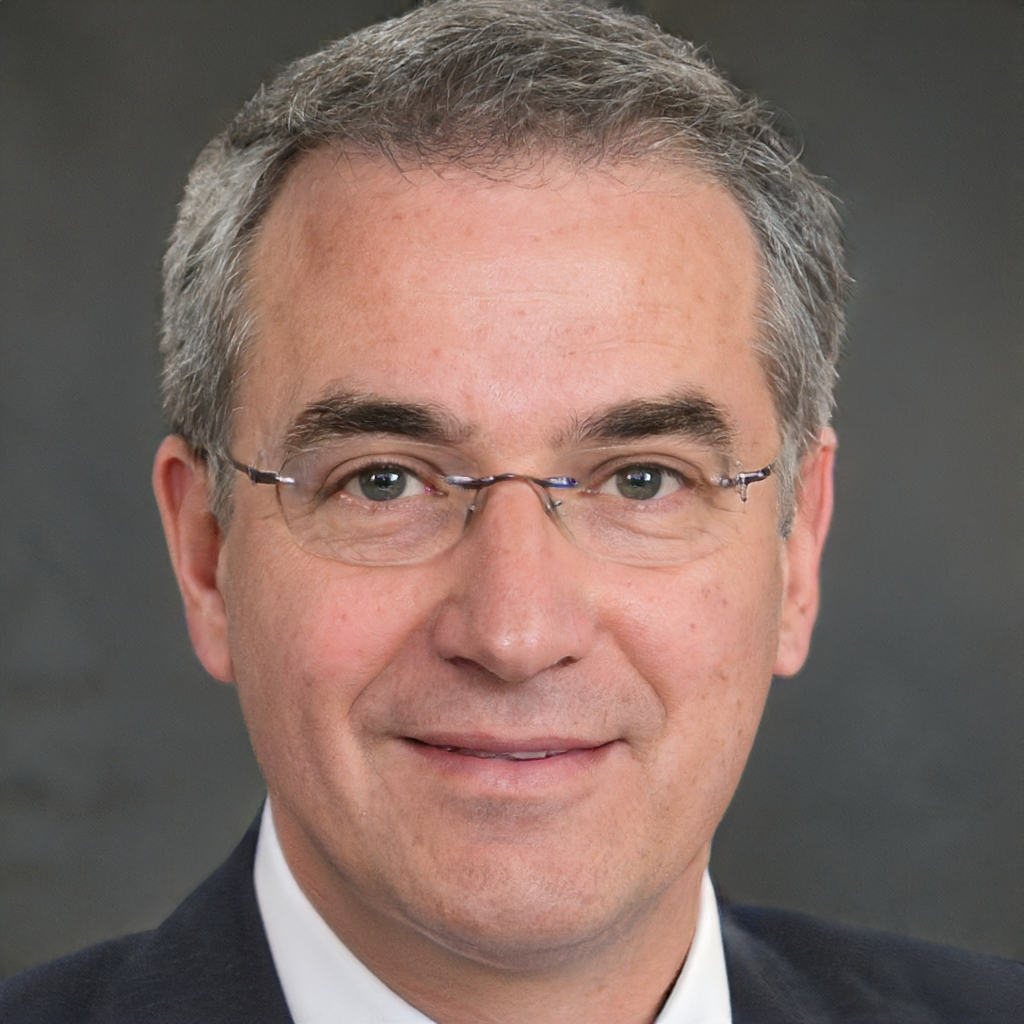
\includegraphics[width=0.24\textwidth]{1.jpeg}
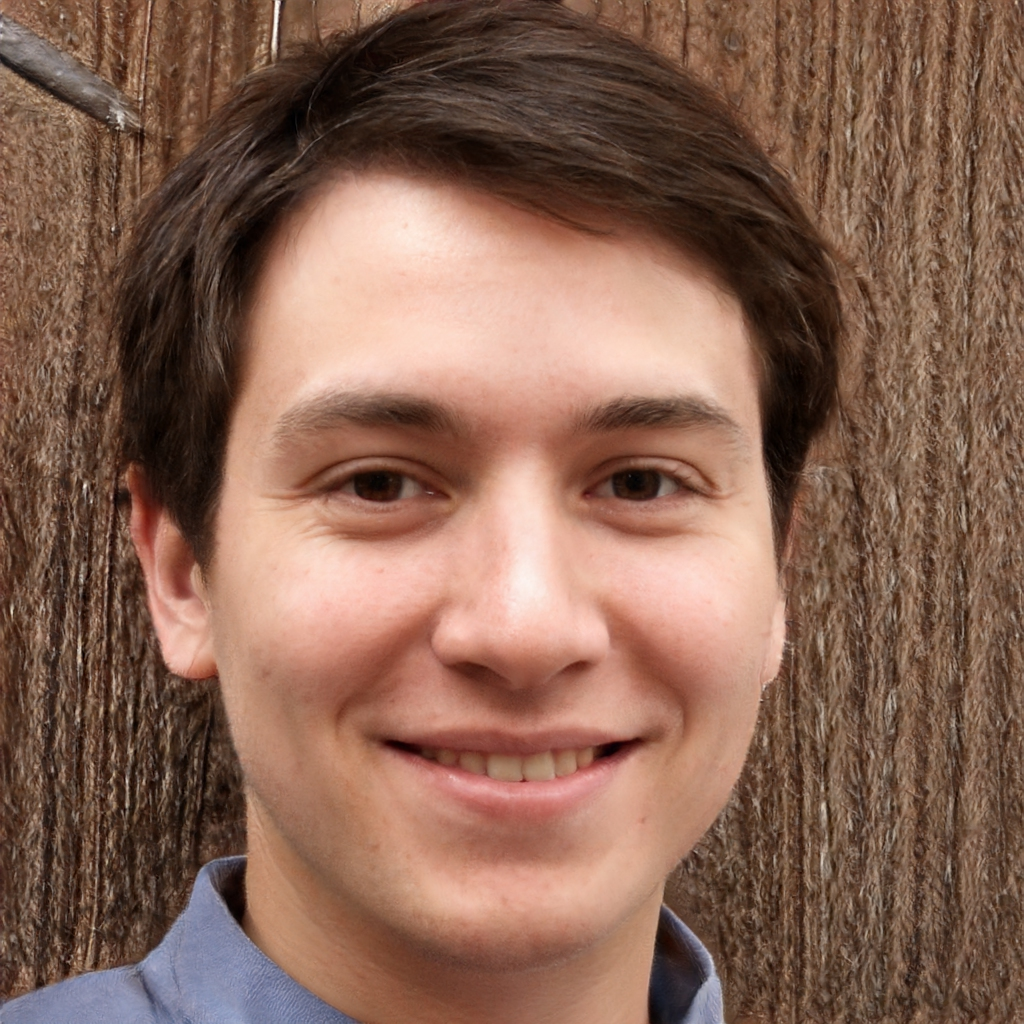
\includegraphics[width=0.24\textwidth]{2.jpeg}
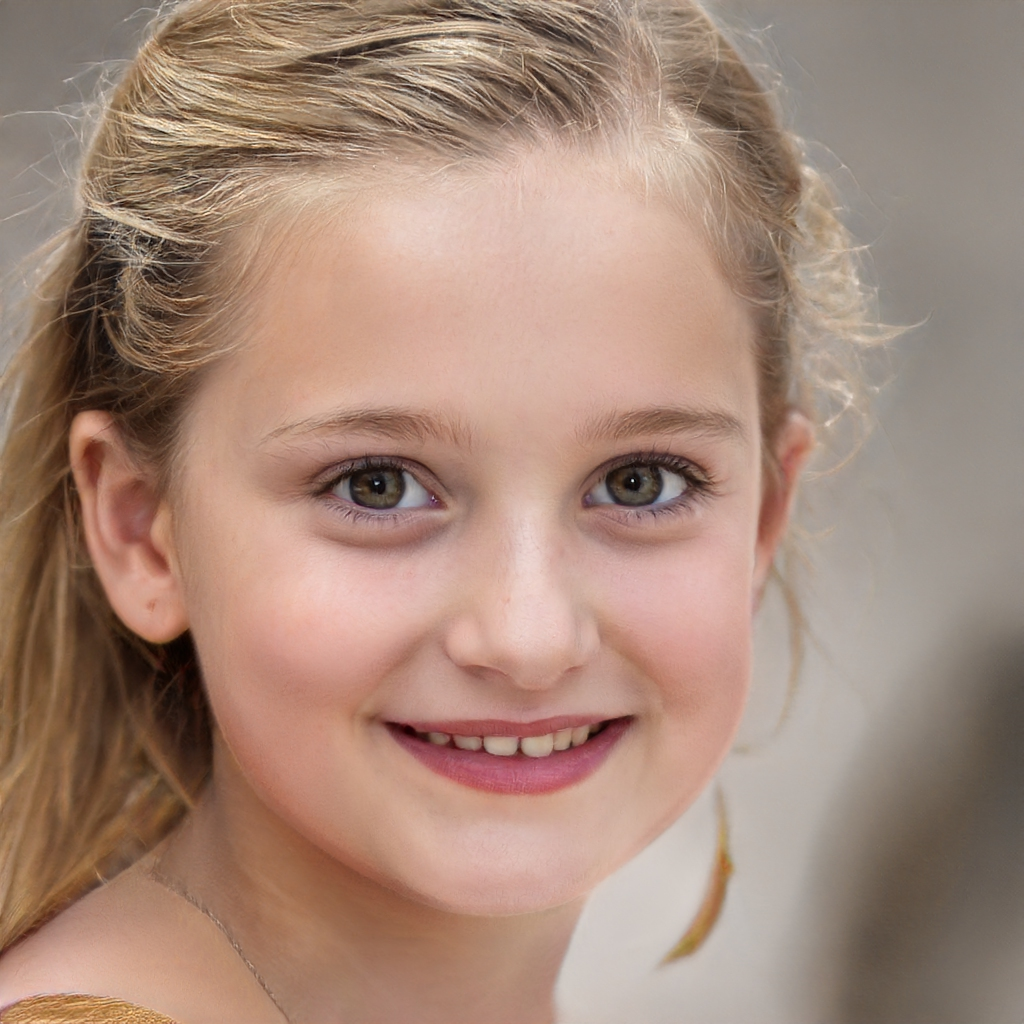
\includegraphics[width=0.24\textwidth]{3.jpeg}
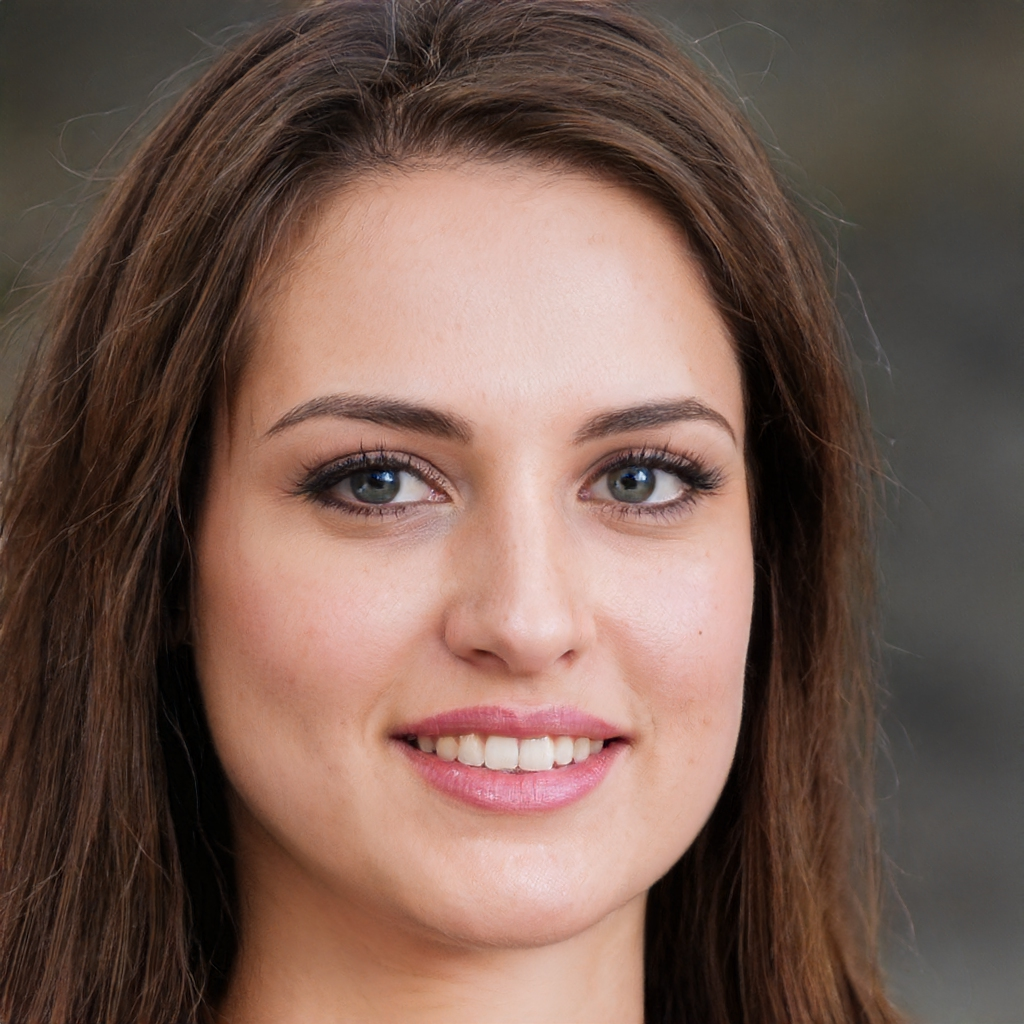
\includegraphics[width=0.24\textwidth]{4.jpeg}
\centering
\caption{Volti di persone (inesistenti), generati da styleGAN.}
\end{figure}
\section{Minimax GAN}
La struttura di una GAN tradizionale è abbastanza semplice: vi sono due reti che "giocano" una alla volta, una contro l'altra. Una rete $D$ (detta discriminatrice) viene allenata a distinguere le configurazioni reali da quelle generate dall'avversaria; subito dopo l'altra (detta generatrice, $G$) viene allenata ad ingannare la rete discriminatrice. $D$ viene strutturata in modo da fornire come output la probabilità che un campione sia reale; $G$ invece viene costruita in modo da fornire, a partire da un set $z$ di numeri random con distribuzione $p_z$, un campione simile a quelli del dataset di partenza. Quindi $D$ viene allenata per massimizzare la probabilità $D(x)$ che i campioni reali $x$ vengano riconosciuti come reali e la probabilità $(1-D(G(z)))$ che i campioni fake $G(z)$ vengano riconosciuti come fake, mentre $G$ viene allenata in modo da minimizzare la probabilità $(1-D(G(z)))$ che i campioni fake vengano riconosciuti come tali.\\
Ogni step del training avviene dunque secondo il seguente schema:
\begin{itemize}
\item Si selezionano N campioni reali $x$ (ossia un mini-batch) e si estraggono N vettori random $z$;
\item Si genera un mini-batch di campioni fake: $G(z_1), ..., G(z_N)$;
\item Si aggiornano i pesi del discriminatore usando come loss function: 
\begin{equation}
\frac{1}{N}\sum_{i=1}^{N} [-\log(D(x_i)) - \log(1-D(G(z_i)))] \,;
\end{equation}
\item Si aggiornano i pesi del generatore usando come loss function: 
\begin{equation}
\frac{1}{N}\sum_{i=1}^{N} [\log(1-D(z_i))] \,.
\end{equation}
\end{itemize}
Per il discriminatore questo metodo corrisponde a minimizzare la crossentropia tra la distribuzione "vera", che associa 1 ai campioni reali e 0 ai campioni fake, e la distribuzione "appresa" che è costituita dall'output del discriminatore stesso. \\
Una interessante interpretazione di questo schema di training è legata alla teoria dei giochi. L'allenamento infatti si può intendere come un gioco non cooperativo di tipo minimax tra le due reti $D$ e $G$:
\begin{equation}
\min _{G}\max _{D}\mathbb {E} _{{\boldsymbol {x}}\sim p_{data}({\boldsymbol {x}})}[\log D({\boldsymbol {x}})]+\mathbb {E} _{{\boldsymbol {z}}\sim p_{\boldsymbol {z}}({\boldsymbol {z}})}[\log(1-D(G({\boldsymbol {z}})))] \,.
\end{equation}
Se la struttura dei dati e delle due reti lo permette, l'obiettivo ideale del training di una GAN classica è raggiungere un equilibrio di Nash
\cite{Nash48}, ossia un punto nel quale entrambe le reti si trovano in una configurazione di pesi dalla quale non hanno alcun vantaggio ad allontanarsi . A quel punto il discriminatore non è capace di distinguere i campioni reali da quelli fake e dà in output il $50\%$ di probabilità in entrambi i casi; le loss valgono quindi:
\begin{align}
D_{loss} = - \log(0.5) - \log(1 - 0.5) = \log(4) = 1.386 \,,\\
G_{loss} = \log(1- 0.5) = - 0.693 \,.
\end{align}
Va notato che molto spesso l'equilibrio non si raggiunge, se non in casi molto semplici, poiché ci si limita a aspettare che il comportamento delle reti diventi stabile e che il generatore crei campioni realistici.
\section{Non-saturating GAN}
\label{Non-saturating GAN}
Nell'articolo originale di Goodfellow\cite{goodfellowgan} in cui si introdussero le GAN oltre alla loss di tipo minimax venne delineato un altro tipo di loss, che secondo gli autori possedeva migliori proprietà di convergenza.
La differenza con la minimax consiste nel massimizzare (per il generatore) la probabilità che i campioni fake vengano riconosciuti come reali, piuttosto che minimizzare la probabilità che vengano classificati come irrealistici. Dunque 
\begin{equation}
G_{loss} = - \mathbb{E}_{z \sim p_z} \log(D(G(z)) \,.
\end{equation}
Uno dei motivi per cui si preferisce questa loss è che tende a saturare di meno quando i campioni fake sono molto poco realistici. Per chiarire quest'aspetto, si supponga che la distribuzione $p_{model}$ dei campioni fake e la distribuzione reale $p_{data}$ siano due gaussiane 1D centrate in punti diversi $m$ e $d$. La loss minimax del generatore diventa costante lontano da $d$, quindi il generatore non riesce ad apprendere nulla a causa dell'azzeramento dei gradienti. Con la non-saturating loss la situazione si inverte.
\begin{figure}[H]
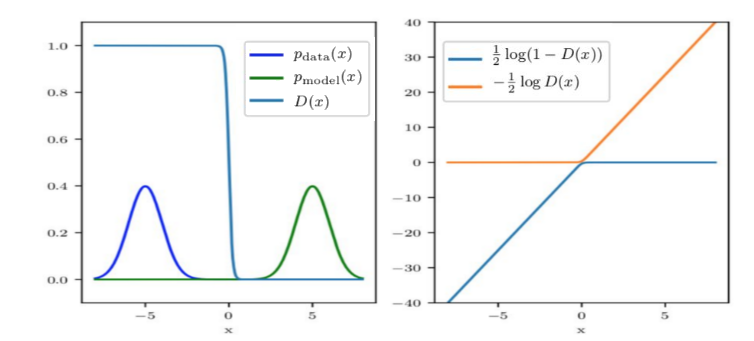
\includegraphics[scale=0.5]{non-saturating-GAN.png}
\centering
\caption{Confronto tra non-saturating e minimax loss nel caso gaussiano 1D \cite{manypathsgan}. Per l'output del discriminatore $D(x)$ si è supposto un andamento sigmoideo, dal quale si deduce il comportamento delle loss.}
\end{figure}
\chapter{Sviluppo della DCGAN}
\section{Dataset}
Il dataset utilizzato per allenare le reti è stato fornito gentilmente dal prof. S. Giagu. Esso è stato ottenuto con l'algoritmo di Metropolis e consiste in 10k configurazioni con temperatura da 0 a 5. Il dataset, a causa di una termalizzazione leggermente incompleta, presenta due caratteristiche che saranno processate in modo diverso dalla GAN. Come si vede in figura \ref{difetti}, vi è infatti la ripetizione di un pattern nella prima riga di pixel di quasi tutte le configurazioni e la presenza, nelle configurazioni a bassa temperatura, di bande verticali di spin allineati, corrispondenti in totale all'1\% del dataset.
\begin{figure}[H]
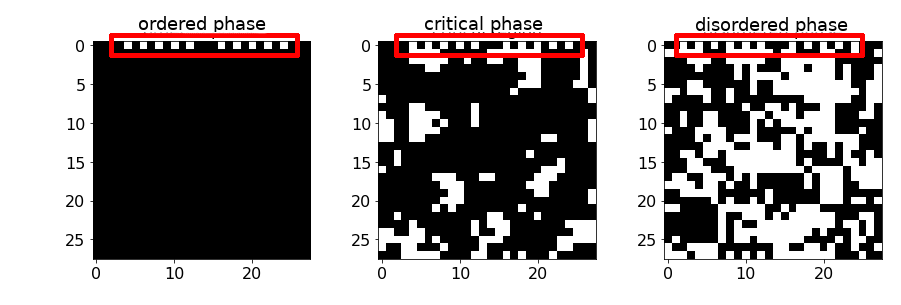
\includegraphics[width=0.8\textwidth]{dataset.png}\\
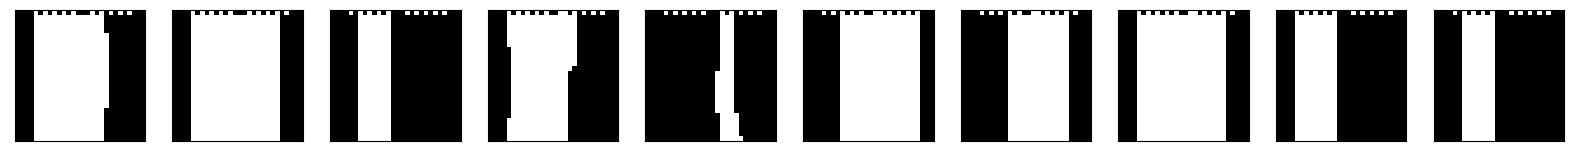
\includegraphics[width=0.9\textwidth]{difetti.png}
\centering
\caption{Visualizzazione delle suddette caratteristiche del dataset}
\label{difetti}
\end{figure}
\section{Topologia delle reti}
Come discriminatore ho usato una rete convoluzionale\footnote{Anche detta CNN, da Convolutional Neural Network.\\ Si veda: \url{https://www.deeplearningbook.org/contents/convnets.html}}, che prende in input le immagini da analizzare $I$ e la classe di temperatura $T$. Il vettore one-hot\footnote{Un vettore one-hot è un versore con una sola componente uguale ad 1 e le altre pari a 0. Normalmente, come in questo caso, l'indice della componente pari ad 1 rappresenta un indice di classe.} $T$ in input viene processato da un layer denso (ossia con tutte le sinapsi tra esso ed il layer precedente attive) e trasformato in una matrice $M$ $(28\times28)$. Successivamente $I$ ed $M$ vengono concatenate ottenendo un'immagine $(28\times28\times2)$ a due canali, che viene passata al primo layer convoluzionale. L'output della rete, invece, è la probabilità che l'immagine in input sia reale e corrisponda alla temperatura indicata.
\begin{figure}[H]
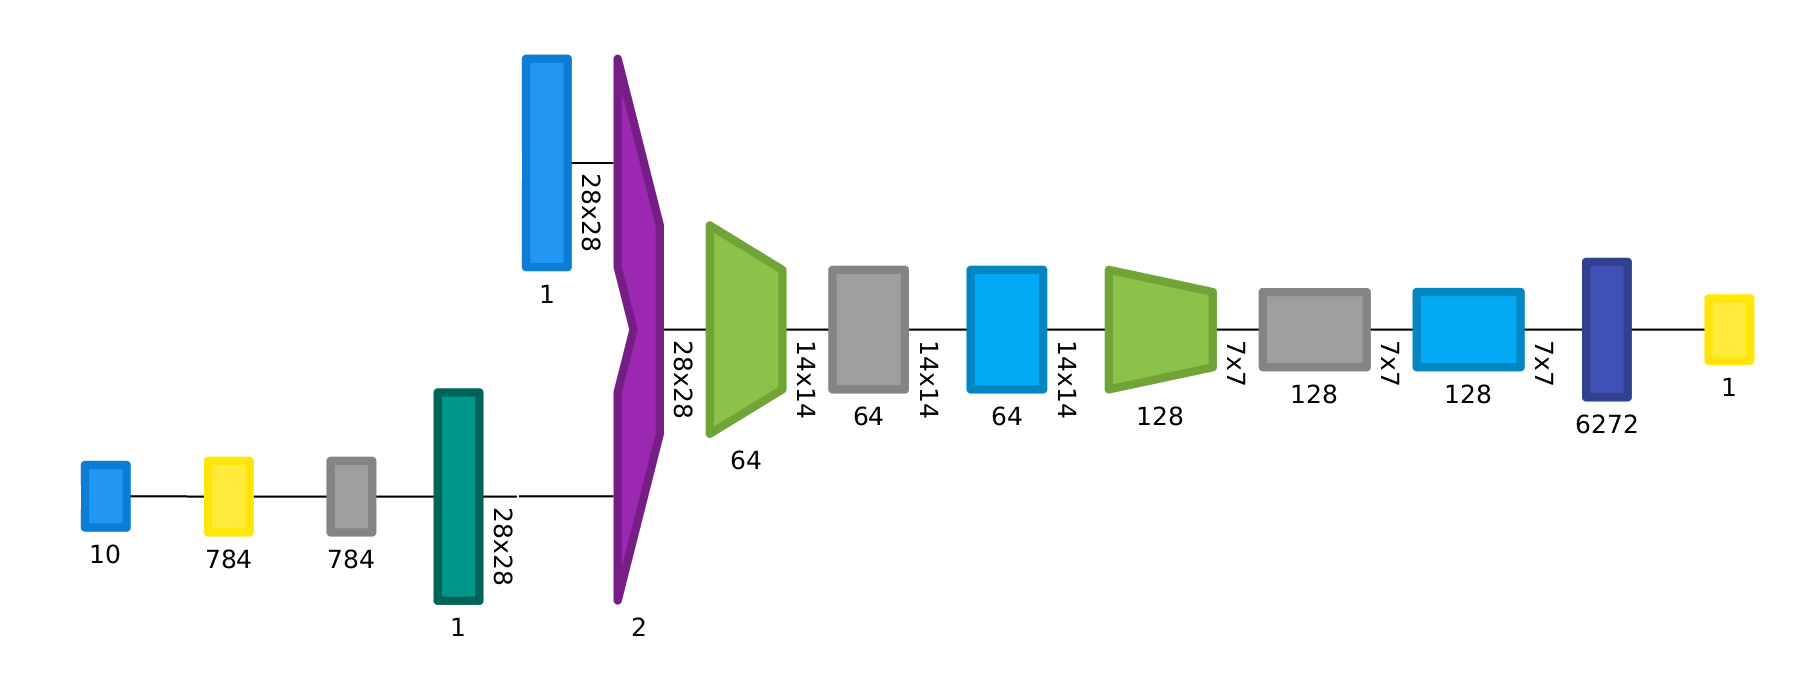
\includegraphics[width=\textwidth]{dis.png}\\
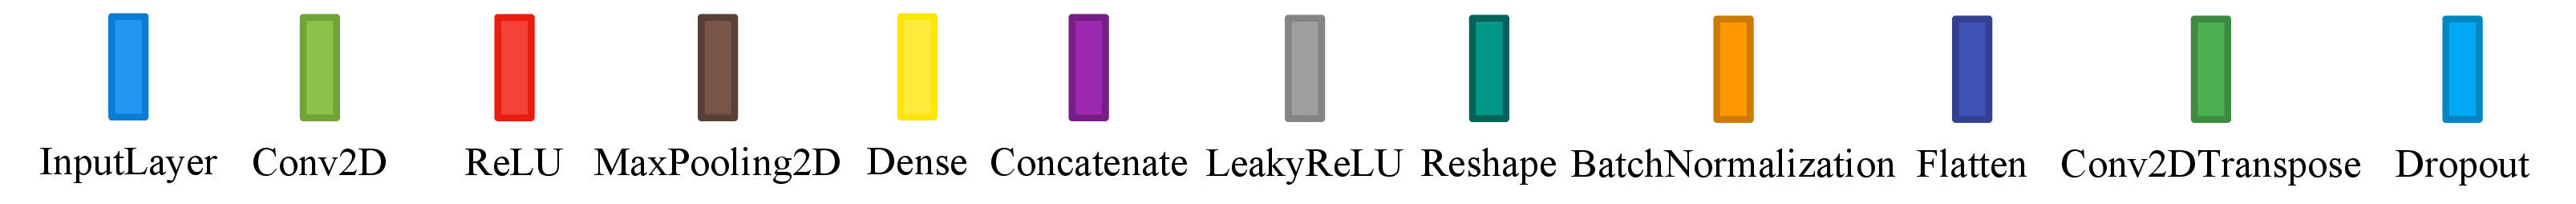
\includegraphics[width=\textwidth]{legend.jpg}
\centering
\caption[...]{Struttura del discriminatore e legenda dei layer utilizzati\protect\footnotemark. In input vi sono un vettore di dimensione 10 (la temperatura in forma one-hot) e l'immagine da processare. Il grafico è stato generato tramite Net2Vis \cite{net2vis}}
\end{figure}

\footnotetext{Per conoscere il funzionamento dei layer utilizzati si veda il glossario al link: \url{https://developers.google.com/machine-learning/glossary}}
Come generatore ho utilizzato una CNN con layer deconvoluzionali, che aumentano la dimensione dell'immagine. L'input è costituito da un vettore random di 128 componenti concatenato al vettore one-hot della temperatura, e l'output (che ha la tangente iperbolica come funzione di attivazione, per dare valori vicini a -1 o 1) da un'immagine 28x28 in scala di grigi.
\begin{figure}[H]
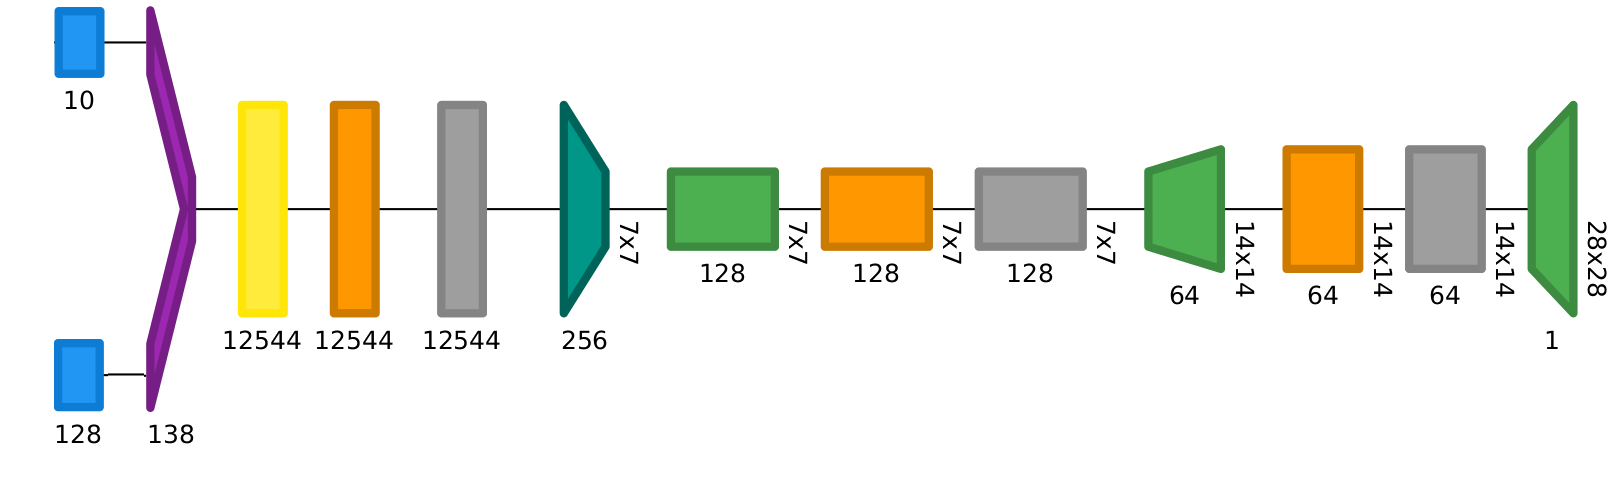
\includegraphics[width=0.9\textwidth]{gen.png}
\centering
\caption{Struttura del generatore. In input vi sono un vettore di dimensione 10 ed il vettore random di dimensione 128.}
\end{figure}
Per aiutare la GAN a prendere decisioni in base alla temperatura, le configurazioni fake vengono date in input al discriminatore insieme alla loro classe di temperatura reale, calcolata da un'apposita CNN, che chiameremo regressore. Essa viene allenata precedentemente rispetto alla GAN e presenta una test accuracy di circa il 65\% (poiché la temperatura può essere predetta in modo affidabile solo intorno alla temperatura critica).
\begin{figure}[H]
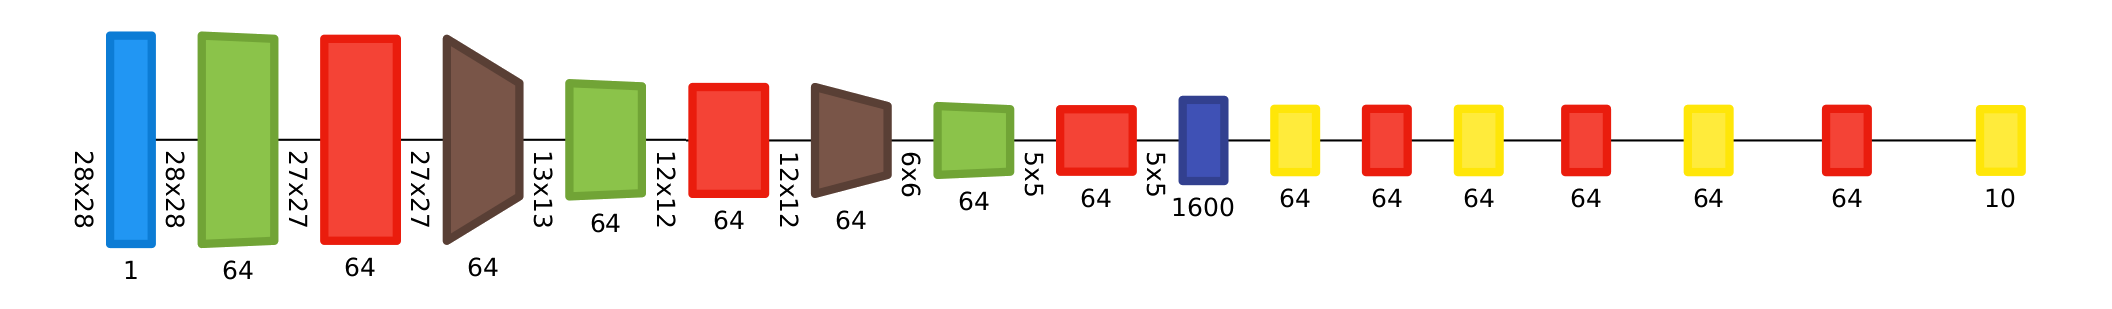
\includegraphics[width=\textwidth]{reg.png}
\centering
\caption{Struttura del regressore.}
\end{figure}
\section{Training schedule}
\subsection{Caso ideale}
\label{Caso ideale}
Il discriminatore $D$ è addestrato minimizzando la crossentropia tra le probabilità in output e le probabilità reali che gli vengono fornite come target. Le coppie di esempi (immagini, classe di temperatura) che gli vengono presentate sono:
\begin{itemize}
\item immagini reali e temperature corrispondenti, con target 1;
\item immagini reali e temperature non corrispondenti, con target 0;
\item immagini fake e temperature corrispondenti (calcolate tramite il regressore), con target 0.
\end{itemize}
In realtà, per aggiungere stocasticità al training, alle label viene aggiunto un rumore uniforme con ampiezza 0.05.
Il generatore $G$ invece viene addestrato massimizzando la probabilità che le configurazioni fake, associate alla temperatura in input, siano riconosciute come reali (cfr. \ref{Non-saturating GAN}).
\subsection{Fasi effettive del training}
Utilizzando questa modalità di training dall'inizio, ho verificato che, sfortunatamente, i gradienti si azzerano dopo poche epoche ed il training si ferma. Osservando il comportamento delle reti dopo questo collasso, ho notato che il discriminatore classificava sempre come corrette le immagini reali, col risultato che il generatore smetteva subito di apprendere. Ho deciso quindi di allenare la GAN partendo dalla schedule tradizionale non-saturating (con l'aggiunta della temperatura) e complicandola progressivamente fino ad arrivare al caso ideale.
Si distinguono tre fasi in base alle coppie di esempi presentate al discriminatore:
\begin{enumerate}[label=\Alph*:]
\item (immagini reali, temperature reali), con target 1;\\(immagini fake, temperature usate per generarle), con target 0;
\item (immagini reali, temperature reali), con target 1;\\(immagini reali, temperature random), con target 0;\\(immagini fake, temperature usate per generarle), con target 0;
\item cfr. \ref{Caso ideale}.
\end{enumerate}
Ho quindi eseguito il training progressivamente con 300 epoche per ciascuna fase, batch size di 64 e usando come ottimizzatore Adam \cite{adam} (con $\eta=0.0002,\,\beta=0.5$, best-practice per le GAN alla Goodfellow).
\section{Processing post-training}
Per aumentare la variabilità dei campioni generati, ho aggiunto al generatore un layer subito prima dell'output che inverte casualmente tutti gli spin con probabilità 1/2. Inoltre ho inserito un layer finale che arrotonda gli output a -1 o 1.
\section{Risultati}
I campioni generati sono abbastanza soddisfacenti: graficamente, come si vede in figura, sono molto simili a quelli generati tramite Metropolis. 
\begin{figure}[H]
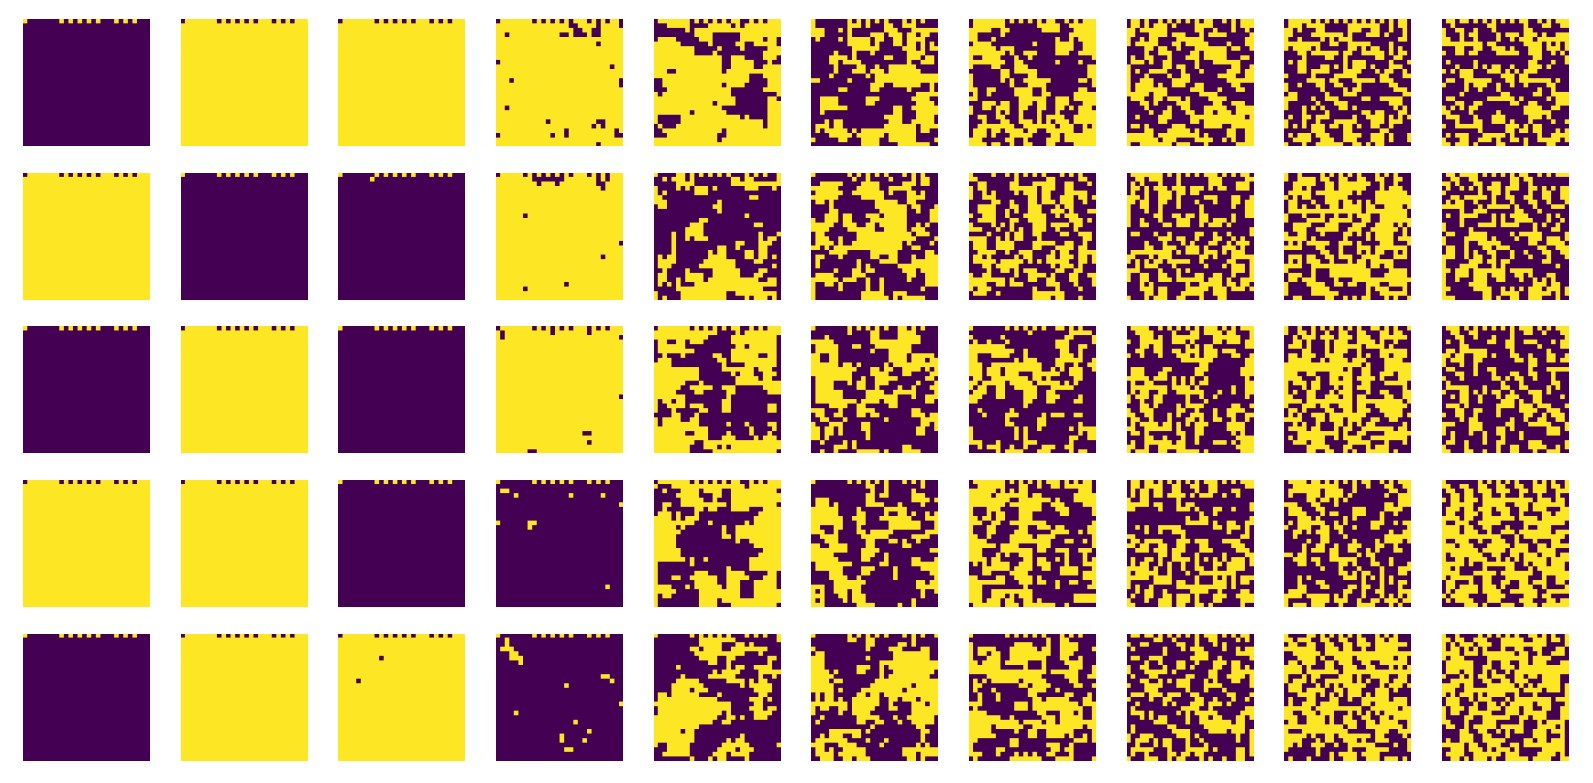
\includegraphics[width=\textwidth]{fig1.png}
\centering
\caption{50 diverse configurazioni generate dalla GAN. I campioni sulla stessa colonna corrispondono alla stessa classe di temperatura, che aumenta da sinistra a destra.}
\end{figure}
Inoltre, come si vede dalla distribuzione della magnetizzazione, la GAN non ha imparato a riprodurre le configurazioni a bande verticali, che erano una caratteristica anomala del dataset (cfr. fig. \ref{difetti}). Questo è probabilmente dovuto al fatto che, dovendo discriminare i campioni anche in base alla temperatura, le configurazioni a bande verticali (che hanno label di temperatura bassa o nulla, ma magnetizzazione piccola) sono percepite dalla rete come anomale. Purtroppo ciò non è avvenuto per il pattern sulla prima riga (cfr. fig. \ref{difetti}), che si ripresenta identico in tutte le configurazioni generate.
Come si vede dallo scatter plot in figura, che contiene 10k punti, la distribuzione della magnetizzazione in funzione della temperatura è molto simile all'originale, a parte per il fatto che non presenta i suddetti difetti a basse temperatura (cfr. fig. \ref{difetti}).
\begin{figure}[H]
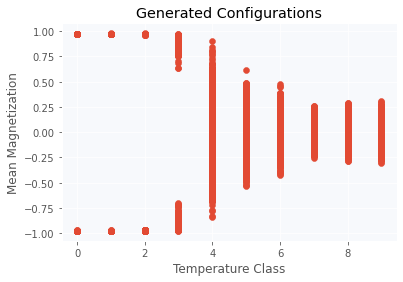
\includegraphics[width=0.49\textwidth]{fakescatter.png}
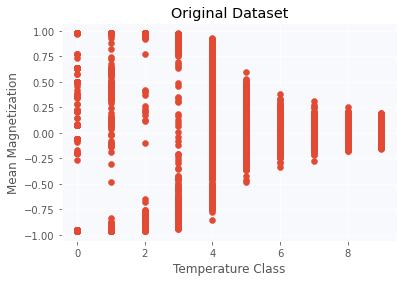
\includegraphics[width=0.49\textwidth]{origscatter.png}
\centering
\caption{Confronto tra campioni fake ed originali dello scatter plot con magnetizzazione vs. temperatura per 10k configurazioni.}
\end{figure}
\begin{figure}[H]
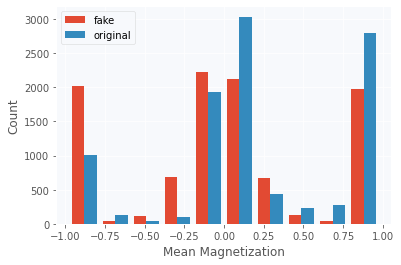
\includegraphics[width=0.7\textwidth]{hist.png}
\centering
\caption{Confronto tra l'istogramma della magnetizzazione dei campioni fake e degli originali.}
\end{figure}
\section{Deployment in JS}
Come demo della GAN sviluppata ho implementato una pagina HTML\footnote{\url{https://raeubaen.github.io/ising.html}} che crea configurazioni del modello di Ising per una data temperatura. La generazione della configurazione avviene sulla macchina del client; ho infatti salvato il modello ed i pesi del generatore da Keras in Python ed implementato il sampling tramite TensorflowJS.
\newpage
\nocite{reference}
\bibliography{bib}{}
\bibliographystyle{unsrt}
\end{document}
